
% ----------------------------------------------------------
% Introdução
% ----------------------------------------------------------
\chapter[Introdução]{Introdução}
Ao observar alguns aspectos da sociedade moderna, os animais domésticos se tornaram figuras essenciais em diversos lares, ocupando o lugar de amigo, filho ou companheiro. Segundo (Ribeiro, 2011)(LINK AQUI) animais domésticos podem trazer sentimentos de lealdade, companheirismo e confiabilidade a humanos que nem sempre são construídos com relações entre indivíduos da mesma espécie. De acordo com (Silva e Marisco, 2018)(LINK AQUI) esses indivíduos quando inseridos na realidade humana, podem trazer diversos efeitos terapêuticos, psicossociais e fisiológicos. \\
 Segundo dados da ABINPET (2021)(LINK AQUI), o Brasil ocupa a sétima posição no Ranking(LINK AQUI) mundial de gastos com animais de estimação. Além disso, no ano de 2019 existiam cerca de 144 milhões de animais domésticos, em sua maioria cães e gatos, e cerca de vinte e cinco por cento do faturamento do ramo Pet é com serviços de Pet(LINK AQUI) Care e Pet Vet. \\
            Com o mundo globalizado, a utilização de Smartphones(LINK AQUI) com aplicativos para tarefas simples vem sendo amplamente difundida pela sociedade. \\
Em uma matéria do Site(LINK AQUI) do governo federal brasileiro (2021) diz: \underline{\textit{“(...)após a popularização desses aplicativos, os consumidores passaram a abrir mão de acessos em diversas prestadoras, tornando-se clientes de uma única empresa(...)”.}} Portanto faz-se necessário que as soluções para tutores de cães e gatos tenham opções seguras e que supram suas necessidades para o cuidado do seu animal. \\
 Tendo em vista que uma das necessidades dos tutores de Pets(LINK AQUI) é o transporte desses seres para consultas, exames, creches caninas, e passeios, este trabalho apresenta, documenta e contextualiza as etapas de desenvolvimento do aplicativo Carrara Pets.\\



\newpage
\section{Objetivos}

\subsection{Objetivo Geral}
O objetivo deste projeto é criar um aplicativo gratuito, de transporte de animais, disponível para celulares  com sistemas Android e IOS,pois são os mais utilizados atualmente.\\

\subsection{Objetivo Específico}
O nosso objetivo específico é que a nossa aplicação funcione de modo similar aos aplicativos de transporte particular humano (UBER, 99, etc.), pois os motoristas com habilitação poderão se credenciar no Carrara Pets(LINK AQUI) e deslocar Pets da subespécie Canis lupus familiaris(LINK AQUI) e da espécie Felis catus(LINK AQUI) com conforto e confiança para os destinos escolhidos pelos clientes.\\
Ter a segurança como uma das nossas prioridades: cães serão transportados utilizando cintos/ cadeiras de segurança e gatos serão transportados em caixas próprias para transporte. Além disso, os carros serão higienizados a cada corrida, os tutores poderão escolher a opção do animal de estimação viajar sozinho ou acompanhado e os motoristas serão avaliados pelos clientes na plataforma.\\


\section{Justificativa}
Atualmente no mercado nacional não encontramos muitas opções de transporte de animais, e os existentes não suprem todas as necessidades de seus usuários, criando assim uma lacuna na melhoria contínua já que não houve muita evolução desses aplicativos.\\
Segundo os dados de 2021 do Instituto Pet Brasil, informa que há cerca de 143,53 milhões de animais de estimação, sendo 58,1 milhões de cachorros, 27,1 milhões de gatos e 58,33 milhões entre outros animais de estimação (INSTITUTO PET BRASIL, 2019 - Gráfico 1).(LINK AQUI)
\begin{figure}
    \centering
    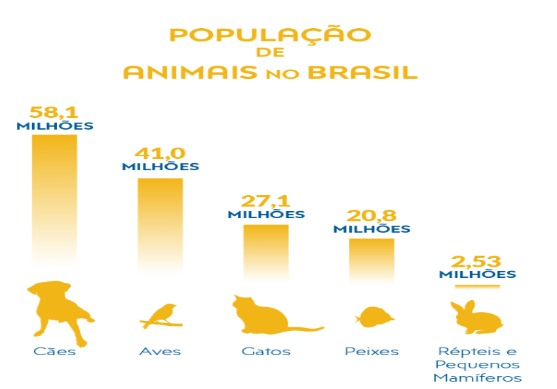
\includegraphics{exemplos/diagramas/População_Animais.jpeg}
    \caption{A população de animais no Brasil no ano de 2021.}
    \label{fig:População_Animais}
    \fonte{Instituto Pet Brasil apud IBGE}
\end{figure}
\\
Considerando o grande número de pessoas com Pets(LINK AQUI) e o carinho que possuem por eles, criou-se   um certo medo de como seus animais serão tratados. Segundo o (Graf , 2016)(LINK AQUI) os donos de animais de estimação, no momento de escolher profissionais para cuidar de seus Pets(LINK AQUI), possuem muitos receios, no que tange a qualidade do serviço e o cuidado do profissional, além disso, o preço do serviço (Gráfico 2)(LINK AQUI).
Um método muito efetivo de conhecer a qualidade de um serviço é por indicação que uma pessoa recebe de um amigo ou conhecido,  nesse âmbito, a aplicação busca disponibilizar avaliações dos parceiros feitas por outros usuários. 
\begin{figure}
    \centering
    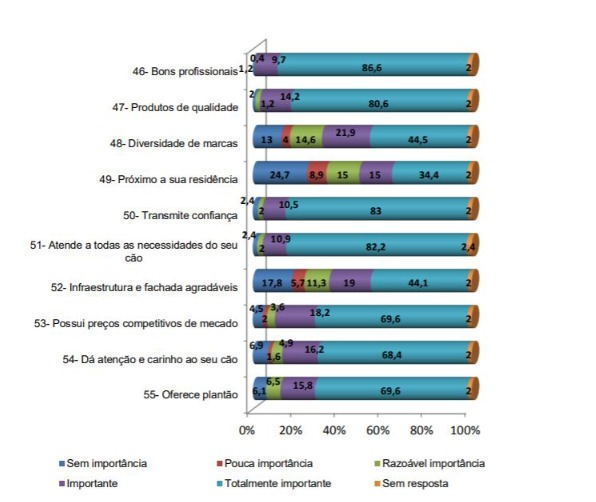
\includegraphics{exemplos/diagramas/graf_analise.jpeg}
    \caption{Principais motivos de escolha de Pet Shops. Os números indicam o número das perguntas, no questionário original da referência Graf (2016)(LINK AQUI)}
    \label{fig:graf_analise}
    \fonte{Graf (2016)(LINK AQUI)}
\end{figure}
\\

\subsection{Análise de concorrência}
Uma das ferramentas importantes no design de projetos é analisar empreendimentos similares e verificar os pontos positivos e negativos para justificar a criação de uma nova proposta. Entre os concorrentes atuais temos:
\begin{itemize}
    \item \textbf{PetDrive:}
        \begin{enumerate}
            \item \textbf{Pontos positivos:}
            Um dos aplicativos mais conhecidos pelo transporte de animais de estimação com seus donos, tendo como um de seus diferenciais o agendamento e equipamentos de transporte de animais dentro do carro disponibilizado pela empresa.
            \item \textbf{Pontos negativos:}
            Não disponibiliza a opção do cliente usar o seu próprio equipamento e não há a opção de viagens de animais desacompanhados.
    \end{enumerate}
    \item \textbf{Uber Pets}:
    \begin{enumerate}
            \item \textbf{Pontos positivos:}
            Conhecido dentro e fora do Brasil, interface intuitiva.
            \item \textbf{Pontos negativos:}
            Os carros não são adaptados para transporte de animais, não transportam o pet sozinho.
    \end{enumerate}
    \item \textbf{Mr. taxidog:}
    \begin{enumerate}
            \item \textbf{Pontos positivos:}
            Empresa antiga  no mercado, com profissionais qualificados e preparados no transporte de cachorros.
            \item \textbf{Pontos negativos:}
            Não é possível transportar outros pets como gatos e pássaros. Funciona somente no estado do Paraná.
    \end{enumerate}
    \item \textbf{Driver dog:}
    \begin{enumerate}
            \item \textbf{Pontos positivos:}
            Empresa com mais de 14 anos no mercado. Possui profissionais qualificados para lidar com cães, e transporte por longas distâncias.
            \item \textbf{Pontos negativos:}
            Não é possível transportar outros seres como gatos, coelhos,etc.
    \end{enumerate}
    \item \textbf{Dog hero:}
    \begin{enumerate}
            \item \textbf{Pontos positivos:}
            Possui profissionais qualificados na área de saúde animal, hospedagem de pets e creche. Está disponível em todo o Brasil.
            \item \textbf{Pontos negativos:}
            Aplicativo pouco intuitivo de transporte com veículo.
    \end{enumerate}
\end{itemize}

Analisando todos os concorrentes vemos que existe espaço para competitividade e crescimento de um novo produto. Portanto, o Carrara Pets busca trazer uma nova experiência para seus clientes , trazendo inovação, facilidade e mais funcionalidades para o cliente e seu pet, não se propondo a só transportar e cuidar dos pets, mas também buscar parcerias que agreguem mais valor para o negócio e satisfação ao consumidor final.

\begin{quadro}[thb]
\centering
\ABNTEXfontereduzida
\caption{Comparativo entre concorrentes}
\label{quadro-poluido-limpo-desalinhado}
\begin{tabular}{|l|l|l|l|l|l|l|}
\hline
\thead{Recursos} & \thead{Pet\\Driver} & \thead{Uber\\Pets} & \thead{Carrara\\Pets} & \thead{Mr.\\Taxidog} & \thead{Driver\\Dog} & \thead{Dog\\Hero}  \\
\hline
Transportar animais & \circlemark & \circlemark & \circlemark & \circlemark & \circlemark & \\
\hline
Corridas agendadas &\circlemark& &\circlemark& & &\circlemark\\
\hline
Serviços prestados pelo motorista & & &\circlemark& & &\\
\hline
Acompanhamento de viagem  &\circlemark&\circlemark&\circlemark& & &\circlemark\\
\hline
Hospedagem & & &\circlemark& & &\circlemark\\
\hline
Creche & & &\circlemark& & &\circlemark\\
\hline
Viagem compartilhada & & & &\circlemark& & \\
\hline
\end{tabular}
\fonte{Os autores.}
\end{quadro}

\section{Estrutura do Documento}
O presente documento está estruturado em 5 capítulos. O Capítulo 1(LINK AQUI), traz a contextualização do tema do projeto e a solução proposta, além de mostrar o objetivo geral e o objetivo específico, que deseja-se conquistar no desenvolvimento da aplicação. Ademais, possui a justificativa para a solução e uma análise de concorrência, demonstrando quais seriam os recursos disponíveis na plataforma Carrara Pets. Para finalizar, o capítulo contém esta seção para explicar a estrutura do documento. \\
No Capítulo 2(LINK AQUI), Revisão da Literatura, reúne-se as referências que forneceram embasamento para o trabalho. Neste capítulo, o leitor contará com temas referentes à aplicativo e público alvo, pontos principais da aplicação.\\
O Capítulo 3(LINK AQUI), Gerenciamento do Projeto, possui seções direcionadas a organização da equipe, falando sobre a metodologia que está sendo utilizada, links que contém algumas informações, como o canal do YouTube, blog da equipe e entre outros. \\
O Capítulo 4(LINK AQUI), Desenvolvimento do Projeto, aborda sobre as tecnologias utilizadas, viabilidade da aplicação, mostra os itens do escopo do projeto, apresenta a arquitetura da aplicação, a modelagem de dados e o diagrama de classes; explica sobre os padrões de projeto, sobre a segurança da informação e outros tópicos referentes ao desenvolvimento da aplicação.\\
Por fim, o Capítulo 5(LINK AQUI) é composto pelo resumo do projeto, explicitando as dificuldades de implementar o Carrara Pets e os obstáculos que apareceram durante o desenvolvimento e as funcionalidades futuras que poderão ser adicionadas à aplicação.\\
Além destes capítulos, o documento contém uma seção de Apêndice, com os documentos extras criados pela equipe ao decorrer do desenvolvimento, que acrescentam informações e melhoram o entendimento do projeto.


\newpage
\section{Processos}
\begin{itemize}
    \item Acompanhamento do veículo 
    \item Diagnóstico do atendimento (Veterinário)
    \item Possível cobrança em casos de compra de remédio
    \item Definição de rota para viagem
    \item Método de fidelidade (Pontos)
    \item Salvar acontecimentos da corrida em forma do tempo
    \item Fidelidade de motorista “X” pet (rotina)
    \item Compatibilidade do porte do pet com dimensões do veículo
    \item Validação do cadastro do motorista (Nome, Idade, Carro, Placa, CNH, CPF, Pré-entrevista com psicólogo(a))
    \item Cadastro de características
    \item Cadastro do pet (Tamanho, Peso, Porte, Temperamento)
    \item Cadastro do dono (Nome, CPF, Idade, Telefone, Endereço...)

\end{itemize}


